% lit. survey II
The description of unbound particles has several complications of conceptual and technical kind.
%Some methods to obtain the FEF had been mentioned in section \ref{ch:r-mat} already, 
In this chapter, different numerical methods are introduced that can be used to solve the one-electron SE in particular for FEFs.
In section \ref{ch:contwa}, the conceptual differences between bound and continuum states as well as the numerical treatment of the latter in a finite basis are discussed.
Thereafter, in the sections \ref{ch:FD} - \ref{ch:wavelet}, different numerical methods are introduced that can be used to solve the one-particle SE on a molecular domain.
%These methods can be roughly divided into two main classes: In section \ref{ch:FD} the finite difference and finite volume methods are introduces which both are based on the approximation of the operators by differences of function values.
%The other methods are based on different basis expansions wich are designed with different properties
%\textcolor{red}{Need to think a bit how to expand on this. Moreover: splines don't fit in there, do they? --> need further category?}
% based on finite differences, a basis-expansion of finite element.

\section{Continuum Waves}
\label{ch:contwa}
Continuum waves are discussed only sparsely in lectures on quantum mechanics, even though their fundamental differences compared to bound states makes them an interesting object to study.
The states considered here have a spatial infinite extend as it is well-known for plane waves 
\begin{equation}\label{eq:PlWave}
\Psi^\text{plan}_{\vec{k}} (\vec{r})=\sqrt{\frac{|\vec{k}|}{(2\pi)^3}}e^{i\vec{kr}}
\end{equation}
with $\vec{k}$ being the wave-vector as well as for spherical waves. %whose radial part contains different powers of $\frac{\sin(kr)}{kr}$ \cite{Lifschitz}.
Moreover, continuum wave functions are not square integrable and hence can not be normalised according to $\int \Psi_{\vec{k}}^\dagger(\vec{r})\Psi_{\vec{k}}(\vec{r}) d\vec{r}=1$ and thus the probability interpretation is invalid \cite{quirky}.
Instead, these functions are sharp in a continuous variable (namely the momentum) and hence should rather be interpreted as probability densities, suggesting the normalisation 
$\int \Psi^\dagger(\vec{r})\Psi(\vec{r'}) d\vec{r}=\delta(\vec{k}-\vec{k'})$ where $\delta(\vec{k})$ is the Dirac delta distribution \cite{quirky,ContOrb}.
This property distinguishes the analytical FEF from those obtained with numerical methods that often have a finite support and are obtained from an approximate Hamiltonian matrix which has no continuous spectrum due to finiteness of its basis.
Especially the difference in the normalisation of wave functions and by this in the dimensionality of overlap integrals also affects the integral evaluated when calculating the transition dipole matrix elements \cite{stieltjesCeder}.
However, the Stieltjes imaging approach described in section \ref{ch:stieltjes} gives a formal verification for the use of square-integrable function for the approximation of a continuum state. %since it can be considered as $0$-th order moment expansion.
Moreover, it provides a formalism to enhance the quality of spectra obtained with numerical methods.

A further aspect of numerical treatment of continuum functions that is only sparsely discussed in literature concerns the question of the physical interpretation of the numerical solution \textcolor{red}{Can one expect some theory about it?}.
When dealing with approximate continuum functions, it is often assumed that the analytic function of interest $|\Psi_\text{a}(\vec{k})\rangle$ is approximated by that particular numeric solution $|\Psi_\text{n}(\vec{k}')\rangle$ which is closest in energy to the desired one \cite{H2pDeCleva} \textcolor{red}{more sources: ideas?}.
An alternative interpretation would be to assume that the numerical solution corresponds to an approximation to $|\Psi_\text{n}\rangle \approx \frac{1}{k^+-k^-} \int_{k^-}^{k^+}|\Psi_\text{a}(k) \rangle dk$ which would change its interpretation and normalisation.
%
%This rises the question, whether a numerically obtained free electron state corresponds most to the analytic state with the same kinetic energy, hence
%$\Psi\approx \Psi_k$
%or whether it should be considered more as an integration over a small part of the spectrum
%$\Psi\approx \frac{1}{k^+-k^-} \int_{k^-}^{k^+}\Psi(k) dk$
%which changes the interpretation and normalisation required for the wave function.

In other works simulating PES in frequency domain only sparsely explicit calculations on the FEF are obtained \cite{ContOrb,H2pDeCleva}.
Instead, mainly two different representations of the photoelectron are found which are based on plane-wave expansions in spherically symmetric bases \cite{ezDyson,DO_TDDFT,do_modCoul}.
One of the expansions is that in spherical waves \cite{Lifschitz}
\begin{equation} \label{eq:spherWave}
\Psi^\text{Sph}_{\vec{k}}(\vec{r})=4\pi
\sum_{l=0}^\infty \sum_{m=-l}^l \text{i}^l j_l\left(kr\right), Y_l^m\left(\theta, \phi\right) Y^{\dagger,m}_l\left(\theta_k, \phi_k\right)
\end{equation}
where $k=|\vec{k}|$ and $r=|\vec{r}|$ are the lengths of the wave vector $\vec{k}$ and spatial vector $\vec{r}$, respectively, $j_l(kr)$ are spherical Bessel functions that solve the radial SE (eq. (\ref{eq:radSEeq}) with $V(r)=0$) and the arguments to the spherical Harmonics $Y_l^m$, $(\theta,\phi)$ and $(\theta_k,\phi_k)$, are the angles of the spherical coordinate system in real-space and Fourier-space, respectively \cite{ezDyson}.
Another expansion of a plane wave often used is that in Coulomb waves
\begin{multline} \label{eq:CoulWave}
\Psi^\text{Coul}_{\vec{k}}(\vec{r})=\frac{1}{(2\pi)^{\frac{3}{2}}}
\sum_{l=0}^\infty \sum_{m=-l}^l \text{i}^l (2kr)^l e^{-\pi\frac{Z}{2k}} \frac{|\Gamma(l+1+i\frac{Z}{k})|}{\Gamma(2l+2)} \\
e^{ikr} F_1(l+1-i\frac{Z}{k}, 2l+2, 2ikr) 
Y_l^m\left(\theta, \phi\right) Y^{\dagger m}_l\left(\theta_k, \phi_k\right)
\end{multline}
where $Z$ is the change of the nucleus and $F_1$ is the confluent hypergeometric function of the first kind \cite{do_modCoul,ColWave} \footnote{$F_1(\alpha,\gamma,z)=1+\frac{\alpha}{\gamma}z + \frac{\alpha (\alpha+1)}{\gamma (\gamma+1)} \frac{z^2}{2!}+\hdots $}.
\begin{figure}
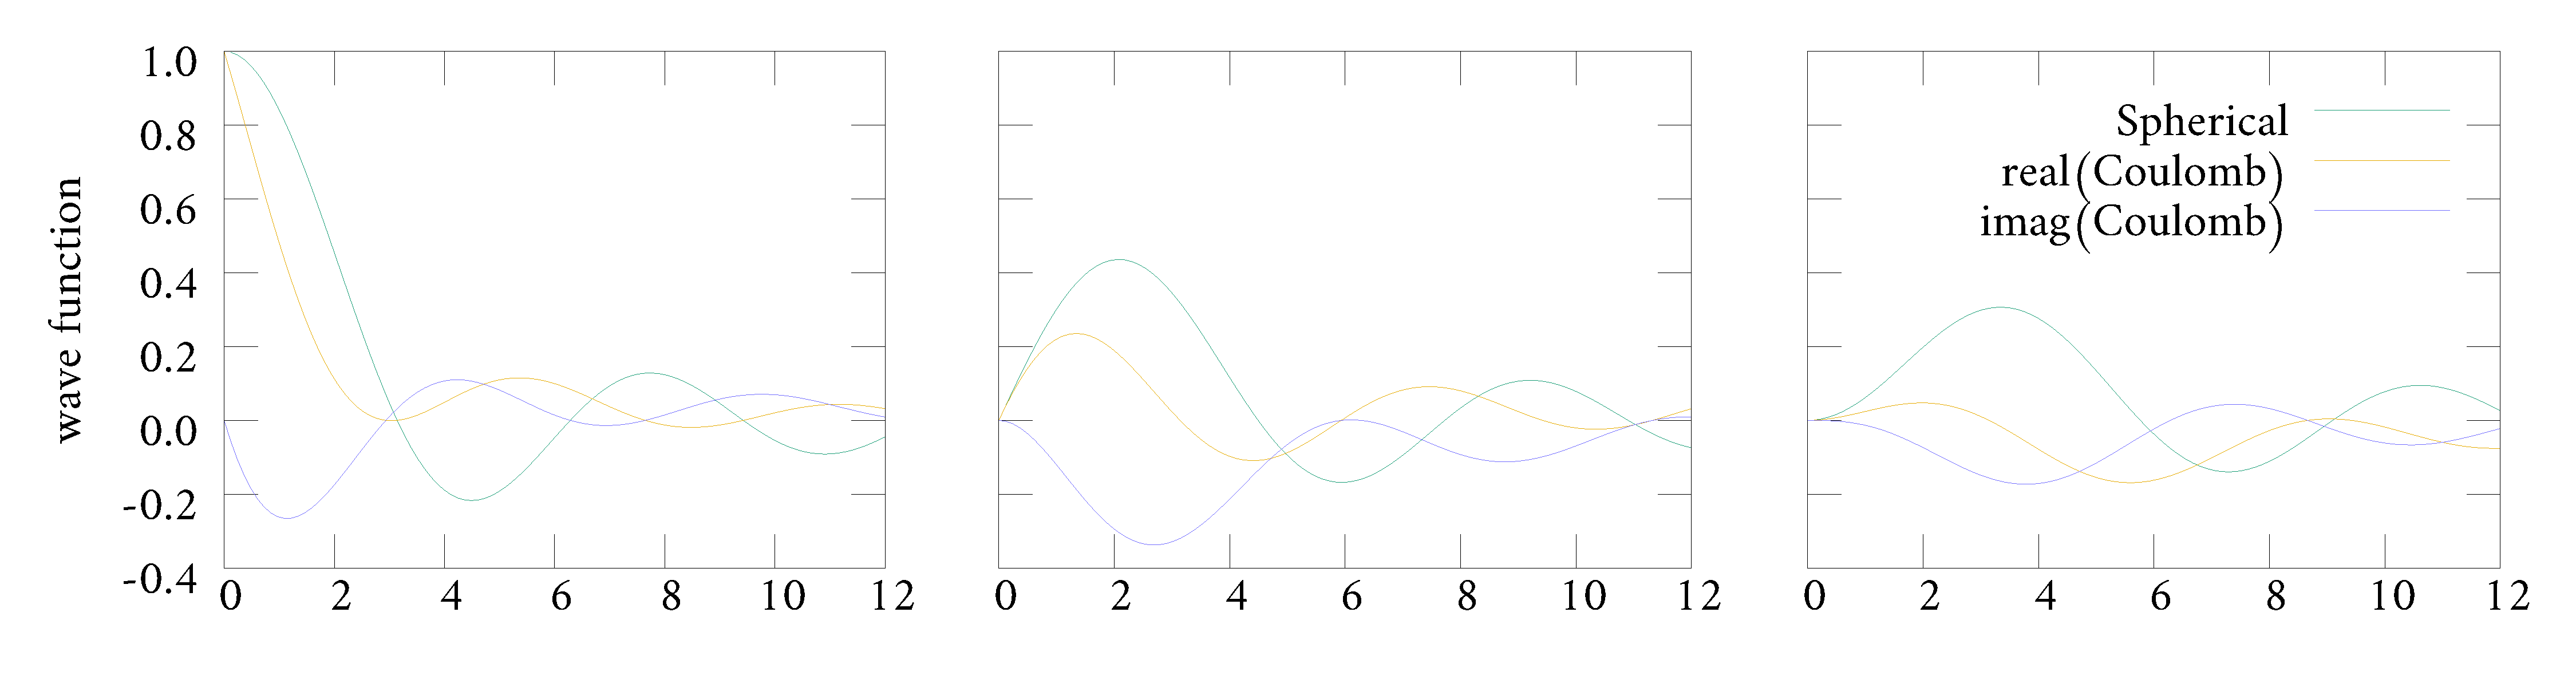
\includegraphics[width=\textwidth]{Figures/RBF/RadialPart}
\caption{Radial part of spherical waves and Coulomb waves (confluent hypergeometric function approximated with 35 terms each) for $l=0$ (left), $l=1$ (centre) and $l=2$ (right).
The Coulomb waves are not normalised.}
\label{fig:RadFun}
\end{figure}

A third expansion that is availible \textit{e.g.} in the program \prog{ezDyson} \cite{ezDyson} is an asymptotic Coulomb wave expression for vanishing momentum in which the confluent hypergeometric function can be approximated by a Bessel function as
\begin{equation}
\lim_{k\rightarrow 0} F_1(l+1+\frac{i}{k}, 2l+2, 2ikr) =(2l+1)! (2r)^{-l-\frac 12} J_{2l+1}(\sqrt{8r})
\end{equation}
where $Z=-1$ is assumed and $J_{2l+2}(x)$ is the Bessel function that is connected to the spherical Bessel functions $j_l(x)$ via the relation $j_l(x)=\sqrt{\frac{\pi}{2x}} J_{l+\frac 12}(x)$ \cite{Lifschitz}.
This case is separately available in \prog{ezDyson} \cite{ezDyson}.

The spherical Harmonics \cite{SphHarm} moreover have the form
\begin{equation}\label{eq:SphHarm}
Y_l^m(\theta,\phi)= (-1)^{(m+|m|)/2} i^l \sqrt{\frac{2l+1}{4\pi}\frac{(l-|m|)!}{(l+|m|)!}}  P_l^{|m|}(\cos(\theta)) e^{im\phi}
\end{equation}
where $P_l^m(x)$ are associated Legendre polynomials \cite{Lifschitz}.
The spherical harmonics are orthonormalised according to
\begin{equation}
\int Y_l^{\dagger m}(\phi,\theta)  Y_{l'}^{m'}(\phi,\theta) d\vec{r}=\delta_{l,l'} \delta_{m,m'}
\end{equation}
and have the property
\begin{equation} \label{eq:dipoleRule}
\int Y_l^{\dagger m}(\phi,\theta) \vec{r} Y_{l'}^{m'}(\phi,\theta) d\vec{r}=\delta_{l,l'\pm 1} C_{l,l', m,m'}
\end{equation}
if not both $l$ and $l'$ are $0$ where $C_{l,l',m,m'}$ are Clebsch-Gordan coefficients.
The relation  (\ref{eq:dipoleRule}) governs the dipole transition probabilities of molecular systems.

Both expansions (\ref{eq:spherWave}) and (\ref{eq:CoulWave}) do not take the molecular potential into account but give an easy picture for the photoelectron.
Since the spherical wave basis is obtained under the assumption of no potential $V(\vec{r})$, this is is assumed to be a good approximation for photodetachement when the initial state is neutral whereas the Coulomb wave expansion takes into account the ESP of the remaining anion at larger distances to the molecule and thus is more reasonable for ionised remainder systems \cite{do_modCoul}.
Due to these obvious deficiencies of the inflexible expansions, some modifications are used by several authors which involve the coise of an effective charge $Z^*<1$ in the expansion (\ref{eq:CoulWave}) \cite{do_modCoul} and an orthogonalisation of the expansion with respect to the DO \cite{do_modCoul,do_orthonorm,do_orthonorm1,do_pworth}.
The latter can be shown to be equivalent to a respective shift of the expansion centre such that the expectation value of the dipole moment of the DO vanishes \cite{do_orthonorm}.

In this work the spherical waves (\ref{eq:spherWave}) are used as reference basis for the computed solutions for an easier interpretation and comparison of different results.
To do so, the numerically obtained solution $|\Psi_\text{n}\rangle$ is projected onto spherical waves for different $l$ and $m$ which will be referred to as partial wave coefficient.
%j_l\left(kr\right), Y_l^m\left(\theta, \phi\right) Y^{\dagger,m}_l\left(\theta_k, \phi_k\right) 

In addition to the previously discussed questions abuot the relation of analytic and numeric FEFs, the infinite degeneracy of the analytical solutions has no numerical counterpart and thus leads to problems which are discussed on the example of the ionisation of a hydrogen-like atom whose analytical FEF is of the form (\ref{eq:CoulWave}) but with arbitrary coefficients for each term whose only prerequisite is that their squares add up to one \cite{Lifschitz}.
%
%In addition to the transition from a continuous to a discontinuous spectrum, also degerarcy plays an important role.
%This can be best discussed when taking the example of the ionisation process of a hydrogen atom where the corresponding FEF has the analytic form

The Coulomb wave basis is, given its energy $E=\frac 12 |\vec{k}|^2$, infinitely degenerate in the direction of $\vec{k}$ as well as in the quantum numbers $l$ and $m$.
%Hence the wave function of a photoelectron can consist of any superposition of the form (\ref{eq:CoulWave}), chosing the coffecients $c_{l,m}$ accordingly.
However, the coefficients of the physically observable FEF are determined by the matrix elements of the dipole operator with the DO (\ref{eq:sigma_do}).
Considering the ionisation of hydrogen in its ground state, the FEF is in one of the three $p$-waves because the probability to access any of the other vaccum-states with the correct energy vanishes due to dipole selection rules eq. (\ref{eq:dipoleRule}) for spherically symmetric systems.

Unfortunately, as shown in section \ref{ch:BCbench}, the considerations made above are not true for the numerical solution anymore where a finite set of superpositions is obtaind which, due to numerical treatment, differ in energy and thus can not be assigned to a common value of $\vec{k}$.
Chosing the energetically best-fitting solution though might in principle result in a function with vanishing contribution of the $p$-type orbitals whereas, for a slightly changed computational schem or target energy it could yield a solution with large $p-$contributions and high intensity, respectively.

%The coefficients $c_{l,m}$ moreover are arbitrary coefficients to this end since any of the linear combinations solves the SE for a given kinetic energy.
%Hence analytical the solutions are not only continuous in $\vec{k}$, but also infinitely degenerate in $l$ and $m$.
%In contrast to this, the numerical solution will be a linear combination of some of these terms; in the easiest case it is close to one of these $l$ and $m$.
%However, for the case of ionisation from the hydrogen ground state only the contributions with $l=1$ will lead to a transition probability; having a solution of $l=2$-character would lead to vanishing probability.
%Hence, the lifting of degeneracy would lead to intensities that are very sensitive to the kinetic energy of the photoelectron since the $l=1$ solution might be only few meV off that solution of $l=2$-type.
%Moreover, the numerical grid may influence this dependency since it could, by accident, supporting certain symmetries.
%
%A detailed discussion of the conceptual complications arising from this is not found in the literature.
%The FEF used to describe the ionisation of H$_2$ as discussed in \cite{H2pDeCleva} is chosen as that function which fits the target energy best.
%However, in their formulation this energy is well-separated from the others % (spline base without boundary conditions, leading to non-hermitian Hamiltonian). -> do they implicitly use some boundary conditions ?
%They also discuss formulation as minimisation problem: More stable but they don't need it.
%which will be later shown to be not the case here.

\subsection{Stieltjes Imaging}
\label{ch:stieltjes}
The Stieltjes imaging \cite{stieltjesCeder,langhoff3,stieltjeLanczos,langhoff} provides an elegant way to use the numerially obtained FEFs of a discrete character lying above the ionisation threshold for PES calculations.% by using moment theory.
To correct on the different character of the spectrum and the smaller extend of the numerically obtained solution, the Stieltjes imaging approach uses spectral moments \cite{langhoff2}
\begin{equation} \label{eq:SpecMom}
\mu_n=\int_0^\infty \epsilon^n df(\epsilon)
\end{equation}
where $n<0$ denotes the order of the moment, $\epsilon=E-E_0$ is the transition energy and 
\begin{equation}
\frac{df}{d\varepsilon}=\frac 23 (E-E_0) \left|\langle \Psi_0 |\vec{\hat{d}}|\Psi_f \rangle \right|^2
\end{equation}
is the oscillator strength with the dipole operator $\vec{\hat{d}}$, the energes $E_0$ and $E$ of the ground state $|\Psi_0\rangle$ and final state $|\Psi_f\rangle$, respectively.
Since the final state can be of bound state character $|\Psi_\alpha\rangle$, where the enegies are discrete, as well as of continuous character $|\Psi_\varepsilon\rangle$ with continuous spectrum, one can rewrite the spectral moment (\ref{eq:SpecMom}) as \cite{langhoff3} 
%Inserting the closure relation $\sum_\alpha |\Psi_\alpha\rangle\langle \Psi_\alpha|+\int |\Psi_\varepsilon\rangle\langle \Psi_\varepsilon| d\varepsilon$ for the full (anatlytic) Hamiltonian results in
\begin{align}\label{eq:M_n_ana}
   \mu_n&=
   %\sum_\alpha \langle \Psi_0 |\hat{d} (\hat{H}-E_0)^n|\Psi_\alpha\rangle\langle \Psi_\alpha| \hat{d} | \Psi_0  \rangle
      %+ \int  \langle \Psi_0|\hat{d} (\hat{H}-E_0)^n|\Psi_\varepsilon\rangle\langle \Psi_\varepsilon| \hat{d} | \Psi_0  \rangle d\varepsilon \\
      \sum_\alpha \left(E_\alpha-E_0\right)^n \left|\langle \Psi_0 | \hat{d}| \Psi_\alpha\rangle \right|^2 + 
         \int_{0}^\infty \varepsilon^n \left|\langle \Psi_0 | \hat{d}| \Psi_\varepsilon\rangle \right|^2 d \varepsilon
\end{align}
where $\varepsilon$ denotes the kinetic energy of the FEF.
%However, inserting the unity expression for the numerical Hamiltonian which does not have continuum functions but an everywhere discrete spectrum and hence $L^2$-integrable eigenfunctions results in
Since, in contrast to the analytic case (\ref{eq:M_n_ana}), the numeric Hamiltonian has a discrete spectrum, the respective spectral moments here are of the form
\begin{equation} \label{eq:M_n_num}
      \mu_n= \sum_{j=0}^N (E_j-E_0) \left| \langle \Psi_0 | \hat{d}| \Psi_j\rangle \right|^2
\end{equation}
where $N$ denotes the number of eigenfunctions $|\Psi_j\rangle$ and the sum accounts for the bound as well as unbound states \cite{stieltjeLanczos,stieltjesCeder}.
%For a good numerical approximation, the expressions (\ref{eq:M_n_num}) and (\ref{eq:M_n_ana}) should be similar for as many $n$ as possible where, due to convergence of the spectral moments, $n<2$ \cite{stieltjesCeder}.
%These considerations are used in the Stieltjes imaging approach with moment theory \cite{langhoff, langhoff2}.
Assuming that the first $2l-1$ spectral moments can be restored by the numerical Hamiltonian in good approximation, they can be used to obtain a histogram representation of the cross section of the form
%In the protocol derived from this scheme thus the oscillator strength $|\langle \Psi_0|\hat{d}|\Psi_\text{el}\rangle|^2$ is approximated by the histogram
\begin{equation}
\sigma(\varepsilon)=\frac 23 \frac{df}{d\varepsilon}
      =\frac 23 \begin{cases} 0 & 0< \varepsilon <\varepsilon_1(l) \\
      \frac 12 \frac{(f_i+f_{i+1})}{\varepsilon_{i+1}-\varepsilon_i}  & \varepsilon_j(n)<\varepsilon<\varepsilon_{j+1}(l)\\
      0   & \varepsilon_n(l)<\varepsilon \end{cases}
\end{equation}
%where $f_i$ is obtained from enforcing the relation (\ref{eq:M_n_num}) for $n=1,\hdots, m$ which is done by solving the matrix equation
where $(\varepsilon_i,f_i)_{i=1,...,l}$ are a principal pseudo spectrum \cite{stieltjeLanczos}. 
The values $\varepsilon_i$ and $f_i$ are obtained from an eigenvalue equation of a symmetric tridiagonal matrix whose diagonal elements $\alpha_i$ and off-diagonal elements $\beta_i$ can be found as parameters a function 
\begin{equation}\label{eq:I_z1}
I(z)=\frac{\beta_0^2}{z-\alpha_1-\frac{\beta_1^2}{z-\alpha_2-\hdots-\frac{\beta_{l-1}^2}{z-a_l}}}
\end{equation}
which contains the full information about the first $2l-1$ spectral moments and has the alternative form \cite{nesbet}
\begin{equation} \label{eq:I_z2}
I(z)=\frac{\mu_0}{z}+\frac{\mu_1}{z^2}+\hdots+\frac{\mu_{2l-1}}{z^{2l}}
\end{equation}
where $\mu_i$ are the spectral moments (\ref{eq:M_n_num}) \cite{nesbet}.
The key task in Stieltjes imaging is the transformation from the form (\ref{eq:I_z2}) to (\ref{eq:I_z1}) \cite{nesbet}.

In practice, the Stieltjes imaging is very demanding if energetically narrow transitions occur since many terms in expression (\ref{eq:M_n_num}) are needed for convergence, making this method efficient mainly for low energy range \cite{H2pDeCleva}.
%Another disadvantage that no asymtotic information about this scheme is reported \cite{H2pDeCleva}.

\section{Finite Differences and Finite Volumes}
\label{ch:FD}
The most common and straightforward approach to solve differential equations such as the SE numerically is via the so-called finite difference (FD) scheme.
Starting from the one-particle SE in atomic units
\begin{equation} 
\left(-\frac 12 \nabla^2 + V(\vec{r}) \right) \Psi(\vec{r})=E\Psi(\vec{r})
\end{equation}
where $V(\vec{r})$ is an arbitrary potential at this point.
Considering a general problem where the low symmetry does not support a product ansatz as \textit{e.g.} eq. (\ref{eq:radSE}) which reduces the dimensionality and thus the complexity of the problem, the kinetic energy operator has in a matrix representation at least $6$ off-diagonal terms per line whose non-banded structure requires iterative solvers \cite{fd_Cart}.
An important disadvantage of finite difference schemes is that they require the evaluation points to be on a regular grid whose stepsize is governed by the sharpest features in the system while local refinement is hardly available.
If considering molecules and thus Coulomb-shaped potentials $V(\vec{r})$, the finest structures are expected to be close to the nuclei whereas at larger distances a respectively dense grid is not needed and thus computations of FEFs with a reasonable box size become very expensive \cite{richardsFD}.
Nonetheless, there are applications of this scheme to the SE \cite{fd_Cart,fd_Cart2}, some of them with massive parallelisation using MPI and multiple GPUs \cite{fd_gpu}.

To overcome this bottleneck for systems with non-uniform parameters, often the finite volume method is used.
The finite volume method is an integral method that is not based on a regular grid.
Instead, for the estimation of the kinetic energy Gau\ss's theorem $\int_V \nabla \vec{u}(\vec{r}) dV=\int_{S} \vec{u}(\vec{r}) \vec{n}dS $ is used where $\vec{u}(\vec{r})$ is a vector-valued function and $\vec{n}$ is the normal vector on the surface $S$ of the volume $V$ under consideration.
Chosing $\vec{u}(\vec{r})=\nabla\Psi(\vec{r})$ yields the relation
\begin{equation} \label{eq:kinFV}
   \nabla^2\Psi(\vec{r})=\lim_{V\rightarrow 0} \frac{ \int_{\partial V} \nabla\Psi(\vec{r}) \vec{n} dS}{V}.
\end{equation}
This scheme becomes especially interesting when the finite volume elements are chosen to be Voronoi cells \cite{Son_Chu0}.
A Voronoi-tesselation is associated with a grid and is constructed such that the Voronoi cell $T_i$ consists of all points in space that are closer to the point $i$ than to any other points in the grid, see Figure {\ref{fig:VorCell} \cite{voronoi,voronoi1,voronoi2}.

This description has the advantage that the quantities on the right-hand side of (\ref{eq:kinFV}) can be associated with properties of the Voronoi-Cell, leading to the first-order approximation of the kinetic energy
\begin{wrapfigure}{l}{0.5\textwidth}
   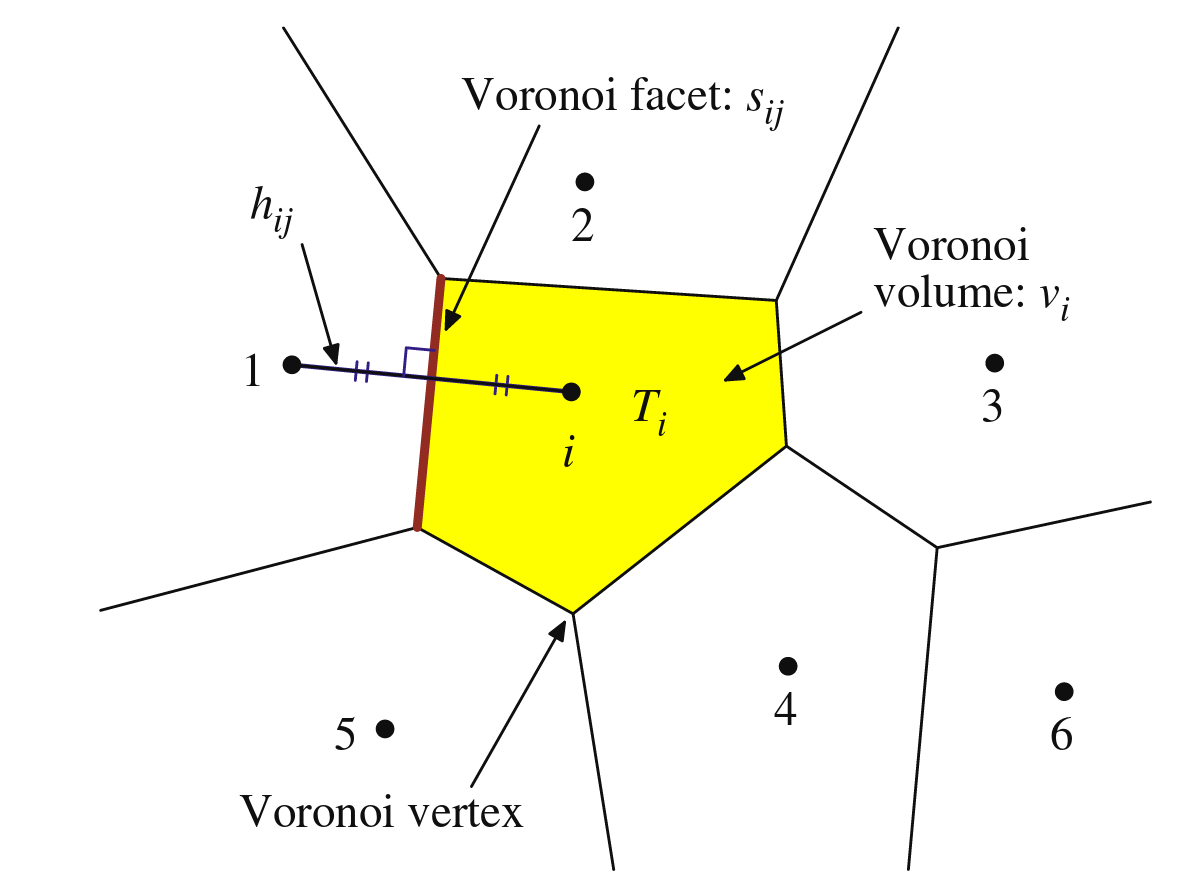
\includegraphics[width=0.5\textwidth]{Figures/VoronoiFD}
   \caption{2-dimensional Voronoi diagram on an arbitrary distribution of seven points \cite{Son_Chu}.}
   \label{fig:VorCell}
\end{wrapfigure}
\begin{equation}\label{eq:kinVoron}
   \nabla^2\Phi(\vec{r}_i)=\frac{1}{v_i} \sum_j^\text{neighbours} \frac{\Psi(\vec{r}_j)-\Psi(\vec{r}_i)}{h_{ij}} s_{ij}a
\end{equation}
where $v_i$ is the volume of the $i$-th Voronoi-cell (yellow area in Figure \ref{fig:VorCell}), $h_{ij}=|\vec{r}_i-\vec{r}_j|$ is the distance between the centres of the $i$-th and $j$-th Voronoi-cells (bolt black line) and $s_{ij}$ is the area of the common facet of the $i$-th and $j$-th Voronoi cells (red line in Figure \ref{fig:VorCell}).

Such a scheme is applied, \textit{e.g.}, by Son and Chu \cite{Son_Chu0, Son_Chu} to the time-dependent SE, studying multi-photon ionisation of several molecular systems.

%\section{Discrete Variable Representation and Splines}
\section{Pseudospectral Methods}
\label{ch:dvr}
Under the term (pse)udospectral methods a large group of methods is comprised which treat the differential equation of interest variationally using an orthogonal basis $\{\varphi_i(\vec{r})\}$, hence seeking for a solution of the form
\begin{equation}
\Psi(\vec{r})=\sum_i^n c_i \varphi_i(\vec{r})
\end{equation}
where $c_i$ are coefficients to be found \cite{SpectMeth}.
In the pseudospectral methods the basis functions $\varphi_i(\vec{r})$ are smooth global functions, \textit{e.g.} $\varphi_{\vec{k}}(\vec{r})=e^{\text{i}\vec{k}\vec{r}}$, resulting in the Fourier space \cite{Fourier}.
Alternatively Jacobi, Chebychef or Legendre polynomials are commonly used \cite{PSbook}.

To find the corresponding coefficients, the problem is solved on a grid, leading to a linear system of equations.
Depending on the technique used for determining the coefficients, it can be seen as a high-order FD or high-order FEM.
One prominent advantage of this class of methods is that the error of the solution $\psi(\vec{r})$ usually decays exponentially with the number $n$ of basis functions and the grid can be chosen coarsely, making the numerical scheme very efficient \cite{PSbook, Tannor}.
In addition, many formulations allow for an implementation making use of the fast fourier transform \cite{PSbook}.

A special representative subgroup of the pseudospectral methods are the so-called discrete variable representation (DVR) schemes which are frequently used to study electronic structure and vibrational problems in molecules \cite{yipDVR,impLDVR,coulDVR}.
Since this scheme is applicable in one dimension only, often symmetry-adapted coordinates such as spherical coordinates are used product functions such as (\ref{eq:radSE}) are applied.

The basis functions used in this scheme commonly are Lagrange polynomials \cite{taoDVR,impLDVR,coulDVR} whose nodes are chosen by a general Gau\ss\, quadrature rule \cite{impLDVR} or from a quadrature rule for the radial Coulomb function which is in particular popular whene electronic structure problems are considered \cite{coulDVR,Tannor}.
Even if the DVR provides a flexible and fast-convergent basis, an extension to higher dimensionality can only be achieved by a product ansatz and thus is applicable to problems with high symmetry.

Moreover, as for the other pseudospectral methods, the system matrices are dense and thus the solution is numerically expensive.
This is at least partially solved by using a hybrid scheme of the finite element and DVR scheme where the DVR scheme is used on small segment only, connected by single bridge-functions each \cite{taoDVR,impLDVR}.

\section{Radial Basis Functions}
The radial basis function (RBF) technique is based on an arbitrary point distribution with very general properties.
The ansatz functions $\varphi_i(\vec{r})$ used in this technique need to be spherically symmetric, \textit{i.e.} $\varphi_i(\vec{r})=\varphi_i(|\vec{r}|)$ and are placed at the grid points on a given domain.
The RBF-scheme is used not only for solving differential equations but is also a usefull tool for interpolation of scattered data in arbitrary dimensions \cite{rbfInterpol} and surface reconstruction from scattered data \cite{rbfSurf}.

Among the commonly used functions are, besides linear and cubic ones, multiquadratic ($\sqrt { r^2 + r_0^2 }$), inverse multiquadratic ($( r^2 + r_0^2)^{-\frac 12}$) and Gaussian ($ \exp(-\frac{r^2}{2r_0^2})$) functions are to be mentioned where $r_0$ is the radius, respectively \cite{rbfSE,rbfWave}.

If the parameter $r_0$ is chosen reasonably, the scheme is numerically stable and fast convergeing \cite{rbfSE}, but the choise of $r_0$ can be non-trivial especially for highly non-regular grids where a good quality of of the representation between two points with a large distance require a respectively large radius $r_0$ whereas too large radii can make the scheme numerically instable for close-lying points.
Moreover the resulting system matrices are dense due to the global definition of the ansatz functions, making it compputationally expensive when large domains are considered.
%Another advantage is the straight-forward implementation and generality of this method.
%\begin{wrapfigure}{r}{0.6\textwidth}
%   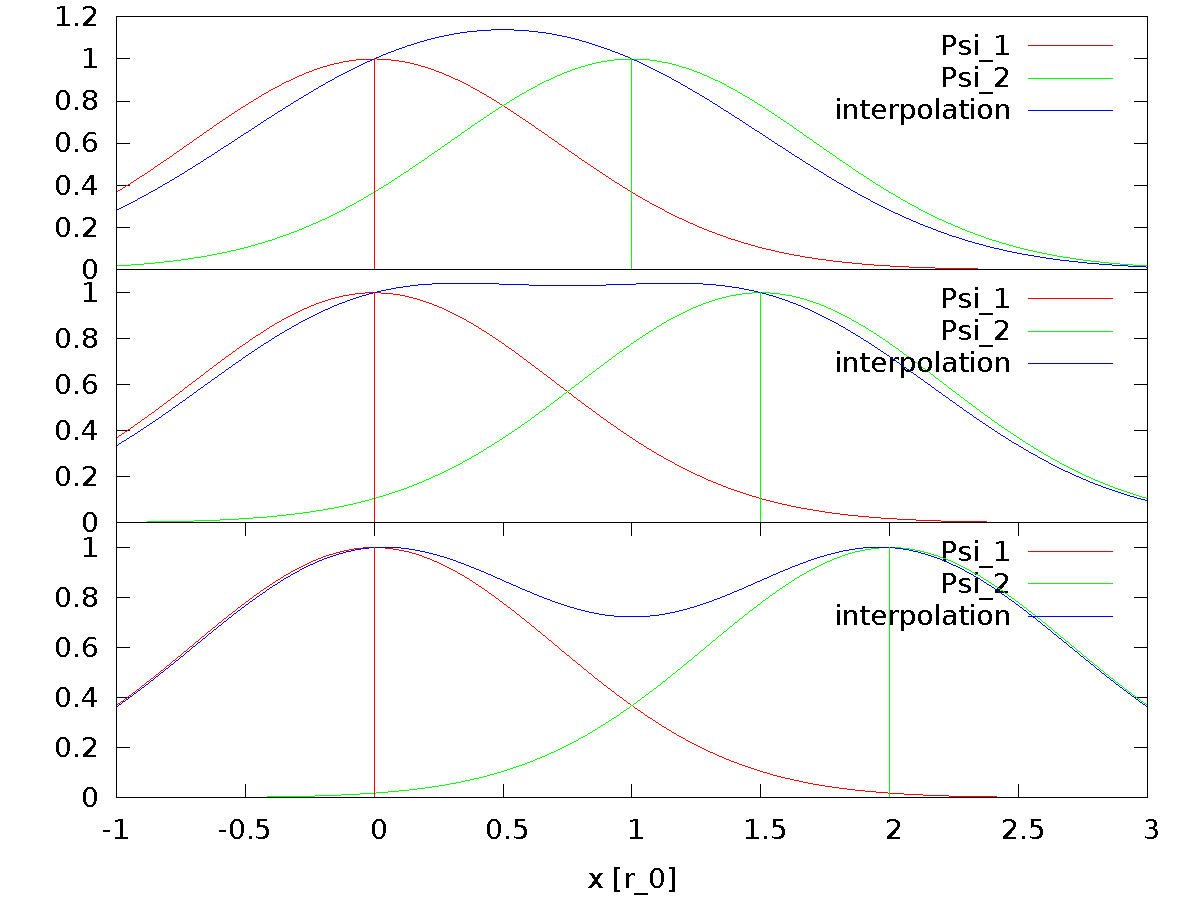
\includegraphics[width=0.6\textwidth]{Figures/RBF/RBFerror}
%   \caption{A function (blue) represented in a RBF basis with Gaussian functions, centred at different distances compared to the broadening parameter $r_0$.}
%   \label{fig:rbfError}
%\end{wrapfigure}
%An important disadvantage of the RBF scheme is that the space between two interpolation points is interpolated non-linearly and, depending on the distance of the two functions, the values are over- or underestimated.
%This error is visualised in Figure \ref{fig:rbfError} for the case of a function that is one at both supporting points, represented by a Gaussian RBF basis.
%The intermediate values of the function depends strongly on the ratio of the broadening $r_0$ and the difference between the supporting points.
%While this behaviour is not problematic for visual purposes, it may introduce a substructure which can lead to unintended behaviour of the solution.

\section{Finite Elements}
\label{ch:introFEM}
In the FEM the differential equations to be solved are formulated in their weak form which is an integro-differential equation and can be understood as a generalisation of the differential equation \cite{femBraess}.
Starting with the well-known (strong) form of the SE defined on a domain $ \Gamma$ in atomic units which are used here and in the following chapters
\begin{equation} \label{eq:SEstrong}
-\frac 12 \nabla^2\Psi(\vec{r})+ V(\vec{r})\Psi(\vec{r})=E \Psi(\vec{r}) \qquad  \vec{r}\in \Gamma
\end{equation}
with the condition 
\begin{equation}
    %\lim_{\vec{r}\longrightarrow \infty} \Psi(\vec{r})=0
    \Psi(\vec{r})=0  \qquad \vec{r} \in \partial \Gamma
\end{equation}
for the boundary domain $\partial \Gamma$ which is assumed to be Lipschitz continuous.
The first term in equation (\ref{eq:SEstrong}) corresponds to the kinetic energy and $V(\vec{r})$ is a potential that is not further specified at this point.
The unknowns of this equation are the wave function $\Psi(\vec{r})$ and respective energy $E$.
To bring equation (\ref{eq:SEstrong}) into the weak form, it is first multiplied by the complex conjugate of a test function $\Phi(\vec{r})$ which fulfils the same boundary conditions and needs to be differentiable.
In the second step, one integrates over the whole space of interest resulting in the equation
\begin{align}
\int d \vec{r} & \left( - \frac 12 \left(\nabla^2\Phi^*(\vec{r})\right)\Psi(\vec{r})
               + V(r) \Phi^*(\vec{r}) \Psi(\vec{r})\right) = E \int d \vec{r} \Phi^*(\vec{r}) \Psi(\vec{r}).
\end{align}
The kinetic energy term can be symmetrised using Green's first identity $\int_\Gamma (\nabla^2\Psi)\Phi^* d\vec{r}=\int_{\partial \Gamma} (\nabla\Psi)\Phi^* ds -\int_\Gamma (\nabla\Psi)(\nabla\Phi^*) d\vec{r}$ to obtain the final expression
\begin{align}\label{eq:SEweak}
\int_\Gamma d \vec{r} & \left(  \frac 12 \left(\nabla\Phi^*(\vec{r})\right) \left(\nabla\Psi(\vec{r})\right) 
               + V(r) \Phi^*(\vec{r}) \Psi(\vec{r})\right) = E \int_\Gamma d \vec{r} \Phi^*(\vec{r}) \Psi(\vec{r})\\
   % &\lim_{\vec{r}\longrightarrow \infty} \Phi(\vec{r})=0.\qquad
   % \lim_{\vec{r}\longrightarrow \infty} \Psi(\vec{r})=0.
    &\Phi(\vec{r})=0\quad
     \Psi(\vec{r})=0\quad  \vec{r}\in\partial\Gamma
\end{align}
which is denoted as the weak form of the SE.
A function $\Psi(\vec{r})$ is considered as a solution of (\ref{eq:SEweak}) if the equation holds for any test function $\Phi(\vec{r})$.
Since usually only real-valued bases functions are used, in the literature the complex conjugation is omitted.
Moreover, from a mathematical point of view, since $\Phi(\vec{r})$ is an arbitrary function, complex conjugation does not change anything here but it will be shown later that it is more reasonable from a physical point of view if the weak formulation is defined as given in equation (\ref{eq:SEweak}).

The weak formulation (\ref{eq:SEweak}) has two main changes in its properties compared to the strong formulation (\ref{eq:SEstrong}).
The first is that any solution of (\ref{eq:SEstrong}) solves (\ref{eq:SEweak}) while the space of solutions of the weak form is larger since only first derivatives need to be defined, which lead to the terms weak and strong respectively.
In addition, a weak solution is defined only up to a cardinal number of zero; hence changing the values of a given solution $\Psi(\vec{r})$ along a finite number of planes in three dimensions yields a function that still solves (\ref{eq:SEweak}).
These properties play an important role here since they allow \textit{e.g.} the use of piecewise linear basis functions as they are commonly used in the FEM scheme which do not have a second derivative and whose first derivative is undefined on certain planes.

As usual for numerical methods, in the FEM scheme one restricts the search for solutions to a subspace spanned by a finite set of test functions for both $\Psi(\vec{r})$ and $\Phi(\vec{r})$, leading to the Petrov-Galerkin scheme.
To get best flexibility for the wave function, the domain $\Gamma$ is subdivided into finite volume elements with a close packing.
These volume elements, denoted as finite elements, give this method its name.
Having this subdivision of space, the ansatz (basis) functions $\varphi(\vec{r})$ used to construct $\Psi(\vec{r})$ and $\Phi(\vec{r})$ are defined as piecewise polynomials being non-zero only on one or few elements.\\
Considering $\Gamma$ to describe a 2D-plane, the elements can be, for example, triangles as shown in Figure \ref{fig:2Del}.
Enumerating the vertices of the triangles as $\vec{r}_i\, i=1,\hdots ,N $, the piecewise linear (Langrange-) basis functions are defined as
\begin{equation}\label{eq:femAnsatz}
   \varphi_i(\vec{r}_j)=
           \begin{cases} 1  & j=i \\
                         0  & j\neq i \end{cases}
\end{equation}
resulting it two-dimensional ``hat'' functions as depicted in Figure \ref{fig:2Del} for an index $i$.
\begin{wrapfigure}{r}{0.75\textwidth}
   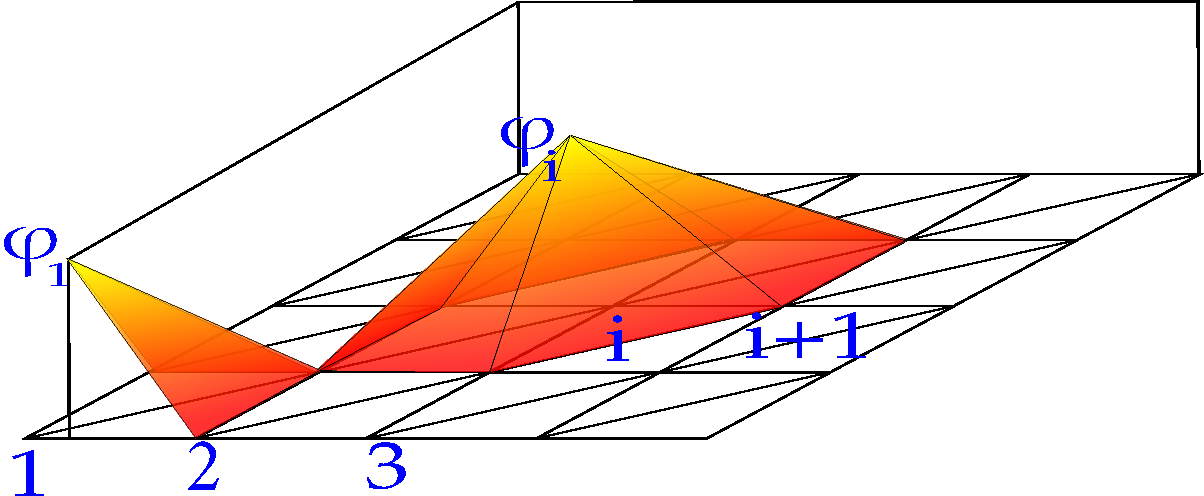
\includegraphics[width=.75\textwidth]{Figures/FEM2d-crop}
   \caption{Example of finite elements in 2D of triangular shape and linear basis functions $\varphi_i(\vec{r})$ defined on them.}
   \label{fig:2Del}
\end{wrapfigure}
This definition of a basis ensures continuity of the solution over $\Gamma$ while the first derivatives are continuous only within each element.
To assure continuity of the first derivatives as well, second order polynomials are needed.
At the boarder of $\Gamma$, respectively truncated ``hat'' functions are used whose coefficients are given by the boundary condition.

As usual in variational schemes, the wave function of interest is constructed as a linear combination of these basis functions $\Psi(\vec{r})=\sum_i c_i \varphi_i(\vec{r})$ where $c_i$ are weighting coefficients.
The test functions are chosen from the same space of ansatz functions, testing each basis separately $\Phi(\vec{r})=\varphi_j(\vec{r}), j\in {1,\hdots, N}$.
Hence, the SE (\ref{eq:SEweak}) with the finite basis reads
\begin{multline}
     \sum_i \int d  \vec{r} \left(\frac 12 \left(\nabla\varphi_i(\vec{r})\right) \left(\nabla\varphi_j(\vec{r})\right) +
                             V(r) \varphi_i(\vec{r}) \varphi_j(\vec{r}) \right) c_i =
               E \sum_i \int d \vec{r} \varphi_i(\vec{r}) \varphi_j(\vec{r}) c_i \\
                      \quad \forall j \in \{1,\hdots ,N\}
\end{multline}
which is the $j$-th component of the generalised matrix eigenvalue problem
\begin{equation}\label{eq:SEmat}
\left(\frac 12 \mat{A} +\mat{V}\right)\vec{c} =E\mat{M}\vec{c}. 
\end{equation}
\text{with}
\begin{align} \label{eq:FEMmatrix}
      \mat{A}_{ij} &=\int d \vec{r} \left(\nabla\varphi_i(\vec{r})\right) \left(\nabla\varphi_j(\vec{r})\right) \quad
      \mat{V}_{i,j}&=\int d \vec{r} V(\vec{r}) \varphi_i(\vec{r}) \varphi_j(\vec{r}) \quad
      \mat{M}_{i,j}&=\int d \vec{r} \varphi_i(\vec{r}) \varphi_j(\vec{r})
\end{align}
and the vector $\vec{c}$ in equation (\ref{eq:SEmat}) contains the coefficients $c_i$ to be found.

The quality of this basis depends strongly on the size and shape of the finite elements:
The stronger the solution varies, the smaller element sizes or higher order ansatz functions are required to be able to represent the wave function.
Knowledge about ranges of sharp structures and areas with smooth variation of the wave function $\Psi(\vec{r})$ hence is crucial for the setup of a good mesh.

In chapter \ref{ch:fem} more details about the finite element formulation are given with a special focus on how to setup a grid that is well suited for describing free particles in quantum mechanics.

\section{Wavelets}
\label{ch:wavelet}
The wavelet method was developed in the 1980s \cite{waveletLA} as a generalisation of the Fourier transform that combines the advantages of the Fourier space and the FEM.
Similar to the FEM, it is based on a local basis but the wavelets have some characteristic scales similar to the wavelength in the Fourier basis, so that they can be used to decompose objects into features of different scales as a generalisation of the Fourier transform \cite{waveletLA, dahlke, FdFeWavelet}.
Even though wavelets posess very advantagous properties, they are to date not very well-established.
The most prominent and widely distributed application of Wavelets is compression of data as used, for example, in the jpeg2000 standard \cite{iso15444}.

%A wavelet is a basis of the function space $L_p(\mathbb{R}^d)$ of functions $\phi(\vec{r})$ for which $\int \phi(\vec{r})^p d\vec{r}<\infty$ which has the form
In general, a wavelet is a basis of the function space $L_p(\mathbb{R}^d)$ \textit{i.e.}, the space of functions $\phi(\vec{r})$ for which $\int \phi(\vec{r})^p d\vec{r}<\infty$ where $\vec{r}\in\mathbb{R}^d$ and $p$ is a positive integer.
A particular wavelet is defined by a finite set of orthonormal mother wavelets $\varphi_i(\vec{r})$ for which a series of functions
\begin{equation} \label{eq:waveBasis}
\varphi_{i,j,\vec{\alpha}}(\vec{r})=m^{\frac{j}{2}} \varphi_i(\mat{M}^j\vec{r}-\vec{\alpha})
\end{equation}
with the matrix $\mat{M}$ whose eigenvalues have modulus larger than one, %(expanding scaling matrix), 
$m=|det(\mat{M})|$ and the running indices $j\in \mathbb{Z}\,$ and $\vec{\alpha}\in \mathbb{Z}^d$ can be defined which span $L_p(\mathbb{R}^d)$ \cite{dahlke}.
%The condition for (\ref{eq:waveBasis}) to be a wavelet basis is that these functionst span $L_p(\mathbb{R}^d)$.
In practice, this very general definition is often restricted by additional requirements such as orthogonality of $\varphi_{i,j,\vec{\alpha}}(\vec{r})$ or utilisation of only one mother-wavelet $\varphi(\vec{r})=\varphi_i(\vec{r})$.
For brevity, in the following only the space $L_2(\mathbb{R})$ with $\mat{M}=2$ is considered which corresponds to the original definition of wavelets \cite{Tasche}.
The most prominent representatives are the Daubechies wavelets that are shown in Figure \ref{fig:wavelets} which are a set of orthogonal wavelets with compact support and increasing smoothness.
Especially the first-order Daubechies wavelet, more commonly known as the Haar-wavelet, is famous and by far the easiest existing orthogonal wavelet basis.
%The most prominent and by far simplest example of a wavelet is the so-called Haar-wavelet wich hase one mother wavelet of the form
%\begin{equation} \label{eq:haar}
%\varphi(x)=\begin{cases} 1 &0\leq x < \frac 12 \\ -1 & \frac 12 \leq x <1 \\ 0 & \text{else}\end{cases}
%\end{equation}
%for which (\ref{eq:waveBasis}) is a orthonormal basis with compact support.
%Another  are the Daubechies wavelets that are a series with  and support.
In contrast to most other bases, in principle no smootheness properties are required but are desired since the functions to be represented are usually smooth \cite{daubechies}.
\begin{figure}
   \begin{subfigure}{0.32\textwidth}
   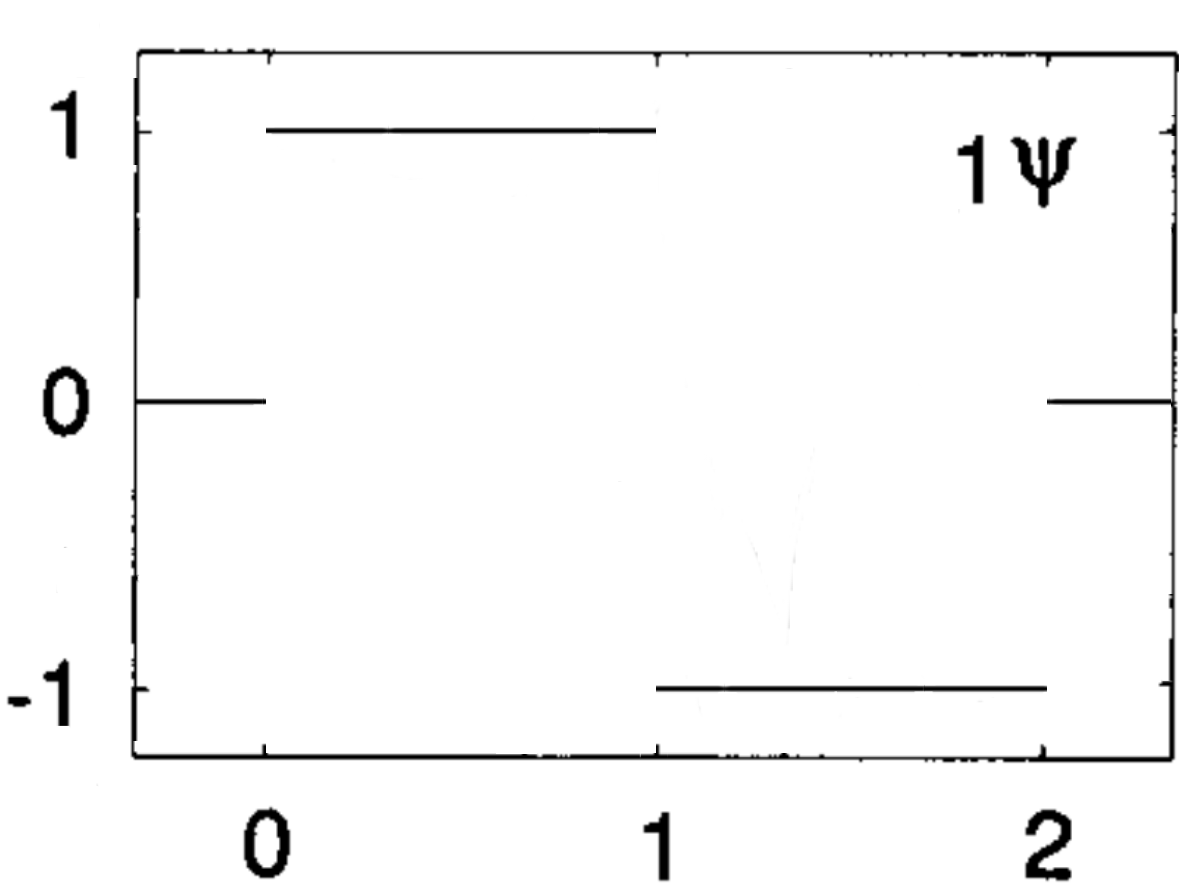
\includegraphics[width=\textwidth]{Figures/Daubechies1}
   \end{subfigure}
   \begin{subfigure}{0.32\textwidth}
   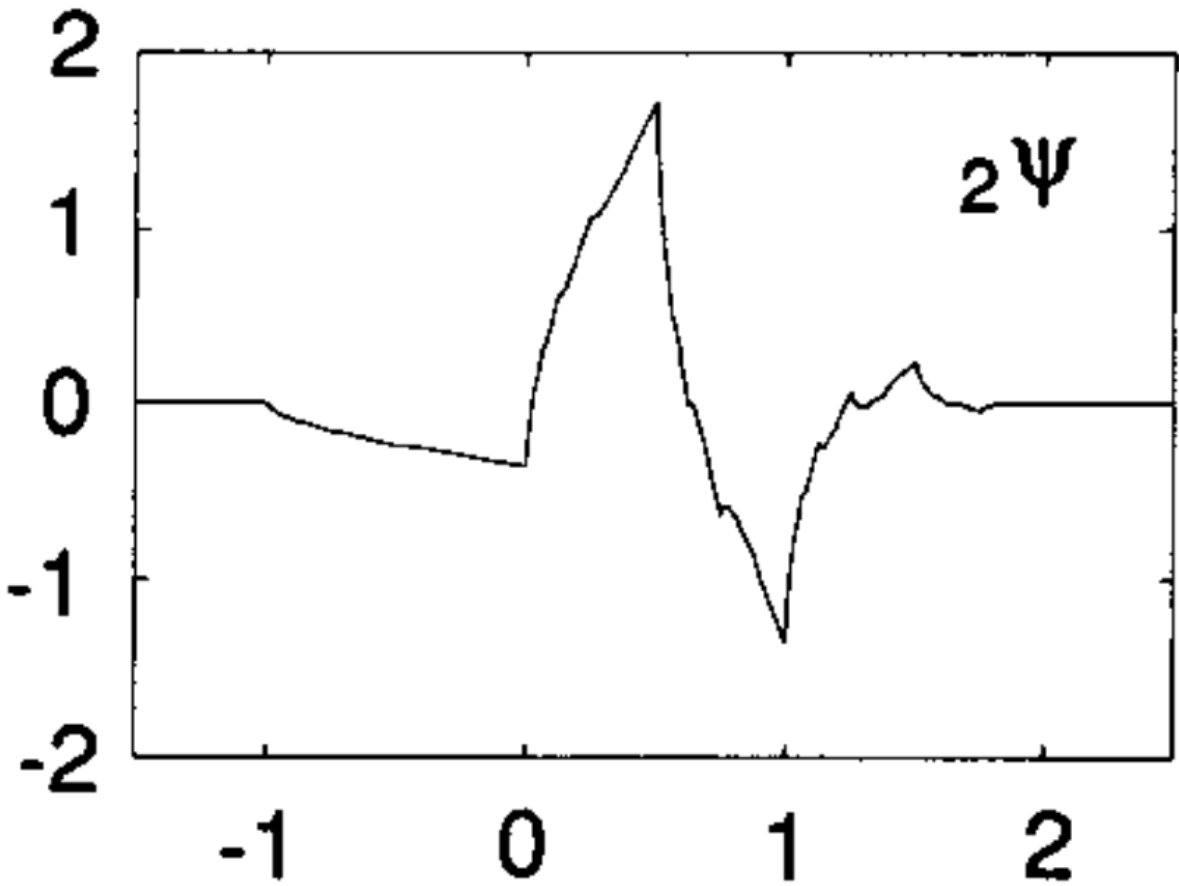
\includegraphics[width=\textwidth]{Figures/Daubechies2}
   \end{subfigure}
   \begin{subfigure}{0.32\textwidth}
   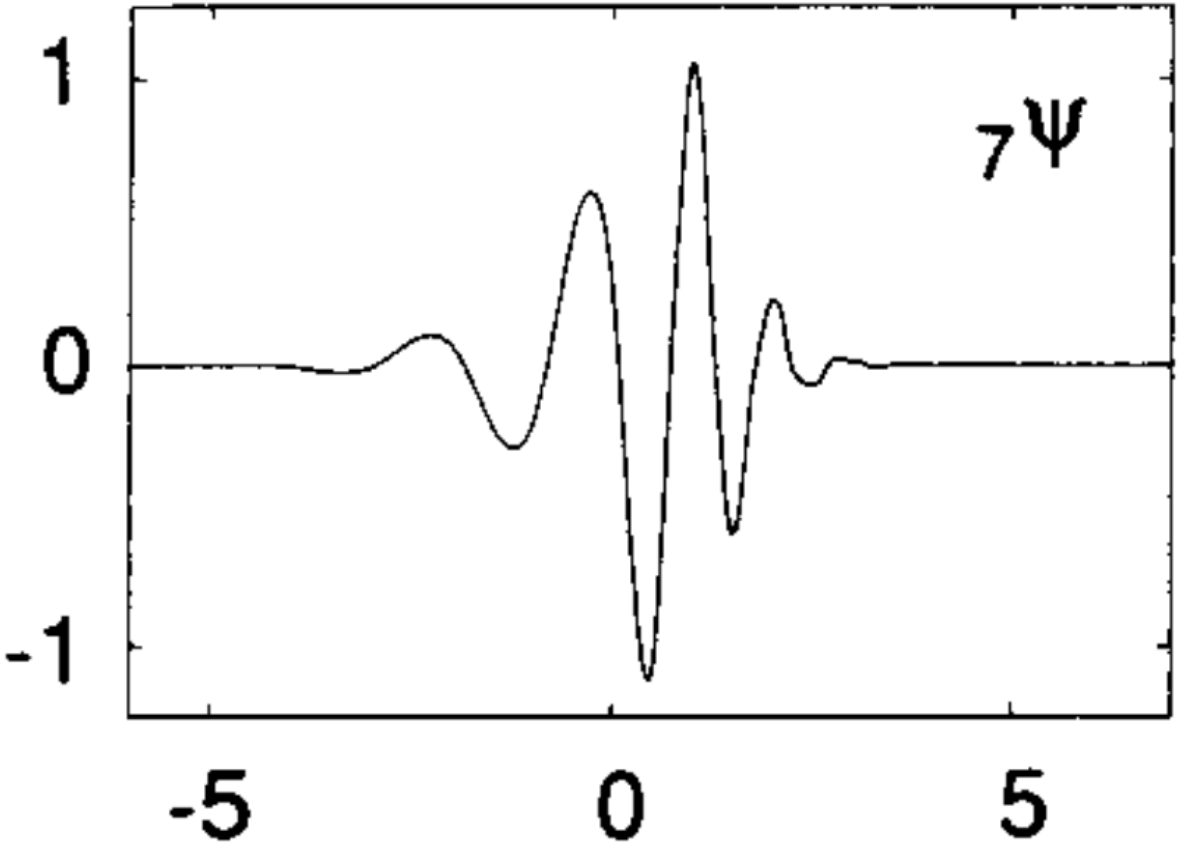
\includegraphics[width=\textwidth]{Figures/Daubechies7}
   \end{subfigure}
   \caption{Daubechies wavelets of the orders 1, 2 and 7 (from left to right) \cite{daubechies}.}
   \label{fig:wavelets}
\end{figure}

Besides their broad use in data compression and analysis, wavelet bases also provide a handy tool to solve partial differential equations and are found to have similar numerical properties as the FEM \cite{FdFeWavelet,CoulWavelet}.
When applying a wavelet basis to solve a partial differential equation, the weak form (\ref{eq:SEweak}) is used \cite{dahlke}.
However, not all wavelets form a valid basis for partial derivatives since, for example, the Haar-wavelet has a constant derivative of zero and the Daubechies-wavelet $2$ (shown in Figure \ref{fig:wavelets}) is only semi-differentiable at some points \cite{WaveletChem}.
However, the generality of the wavelet formulation allows to use problem-specific bases that are, \textit{e.g.}, especially adapted to certain pseudo-differential operators, increasing the speed of convergence \cite{dahlke}.
Finding such optimised bases in a systematic way is under current research and one can expect that they can be used for numerically stable, fast and accurate partial-derivative solvers \cite{dahlke,kunoth}.

\section{Hybrid Methods}
In the previous sections a large variety of different methods are presented with different advantages and disadvantages which make them suitable for different applications.
Moreover, there is a large number of approaches that combine the ideas of some of the above-mentioned methods to use the advantages of the respective methods together.
In this section, several of these methods are presented which seem to be the most prominently used.
One of the most prominent combinations of the above-mentioned methods is the FE-DVR scheme \cite{impLDVR,taoDVR} that was mentioned in chapter \ref{ch:r-mat} already.
%In the FE-DVR scheme, a DVR is used with a set of ansatz functions each defined on a given interval only, referred to as the (1D) finite element.
%A single function connects these intervals similar to the ``hat'' functions in FEM.
In the FE-DVR scheme, a one-dimensional finite element scheme is used with comparatively large elements on which a DVR representation is used, but usually using the strong formulation of the respective partial-derivative equation.
In this approach, more flexibility compared to the DVR scheme is obtained since in addition to the degree of polynomials in use, also the size of the elements can be varied which is especially advantageous for problems involving a Coulomb potential where the local kinetic energy varies strongly \cite{yipDVR}.
Moreover, the usually dense Hamiltonian and overlap matrix of DVR representation changes to a block-structure, with block being coupled to each other by single columns and rows \cite{taoDVR}.
A generalisation to multiple dimensions is the so-called spectral element used by several authors \cite{sem1,sem2,sem3} for quantum mechanical problems.
In contrast to the FE-DVR-scheme, it is based on the weak formulation and typically uses higher order Chebychev or Lagrange polynomials \cite{sem1} and hence allows for larger elements than usual FEM.
Thus, it can be also understood as a high order FEM scheme, combining the flexibility of FEM with the fast convergence of the pseudospectral basis.
The spectral elements are found to be well suited for linear problems but require a complex implementation and lead to denser system matrices.
The larger density in the resulting matrices in general leads to a reduced numerical stability and computationally more expensive solution strategies.
Finally, complex geometries usually benefit more from smaller elements that from higher order bases \cite{hf_dreyer}.

A successfull combination of spectral elements with the FEM is the so-called spectral difference method \cite{SpectDiff,sd_mult}.
In this scheme, a spatially uniform grid is used (as usual in the finite difference scheme) while employing a pseudospectral basis on the respective elements.
The appealing properties of this method are an exponential convergence as known from finite difference methods by employing the sparseness of the equation system obtained in FEM \cite{SpectDiff}.
More advanced methods based on the spectral difference schemes are available as well \cite{sd_mult,sd_unstructured} but are for brevity not discussed here in more detail.

